\begin{frame}{Messprinzip}
  \begin{columns}[c, onlytextwidth]
    \begin{column}{0.47\textwidth}
      \begin{enumerate}
        \item Messung der Doppler-Verschiebung der \SI{21}{\centi\meter}-Linie
          in eine Richtung
        \item Berechne für $v_{\max}$ = maximale Geschwindigkeit:
          \belowdisplayskip=0ex
          \begin{align*}
            R &= R_0 \cdot \sin{γ} \\
            v &= v_{\max} + v_0 \cdot \sin{γ} 
          \end{align*}
        \item Für Milchstraße:
          \begin{align*}
            v_0 = \SI{220}{\kilo\meter\per\second} \\
          R_0 = \SI{8.5}{\kilo pc}
          \end{align*}
      \end{enumerate}
    \end{column}
    \begin{column}{0.47\textwidth}
      \centering
\newcommand{\cloudangle}{18.4349488}
\begin{tikzpicture}
  \draw[thin] (0, 0) circle [radius = 1];
  \draw[thin] (0, 0) circle [radius = 2];
  \draw[thin] (0, 0) circle [radius = 3];
  \filldraw[darkred!30] (0, 3) -- (0, 2.3) arc [start angle=270, end angle=270+\cloudangle, radius=0.7cm] -- cycle;
  \node[fill, anchor=center, black!20,
    cloud, draw, cloud puffs=11, minimum size=0.5cm,
    cloud puff arc=120, aspect=3, inner sep=0em]  at (\cloudangle:1cm) {};
    \draw[darkred, ->, dashed, thick] (0, 3) -- (\cloudangle:1cm) -- +(-90+\cloudangle:3.5cm);  
  \draw (0, 0) -- + (0, 3) node[midway,left] {$R_0$};
  \draw (0, 0) -- (\cloudangle:1cm) node[midway,below] {$R$};
  \filldraw (0, 0) circle [radius=2pt];
  \filldraw (0, 3) circle [radius=2pt] node[above] {Erde};
  \draw[->, thick] (0, 3) -- + (1, 0) node[above] {$v_0$};
  \draw[->, thick] (\cloudangle:1cm) -- +(-90+\cloudangle:1cm) node[right, midway] {$v$};
  \node[left] at (0, 2.65) {$γ$};
\end{tikzpicture}

    \end{column}
  \end{columns}
\end{frame}

\begin{frame}{Die \SI{21}{\centi\meter}-Linie – Vermessung der Milchstraße}%
  \begin{columns}[c, onlytextwidth]%
    \begin{column}{0.47\textwidth}%
      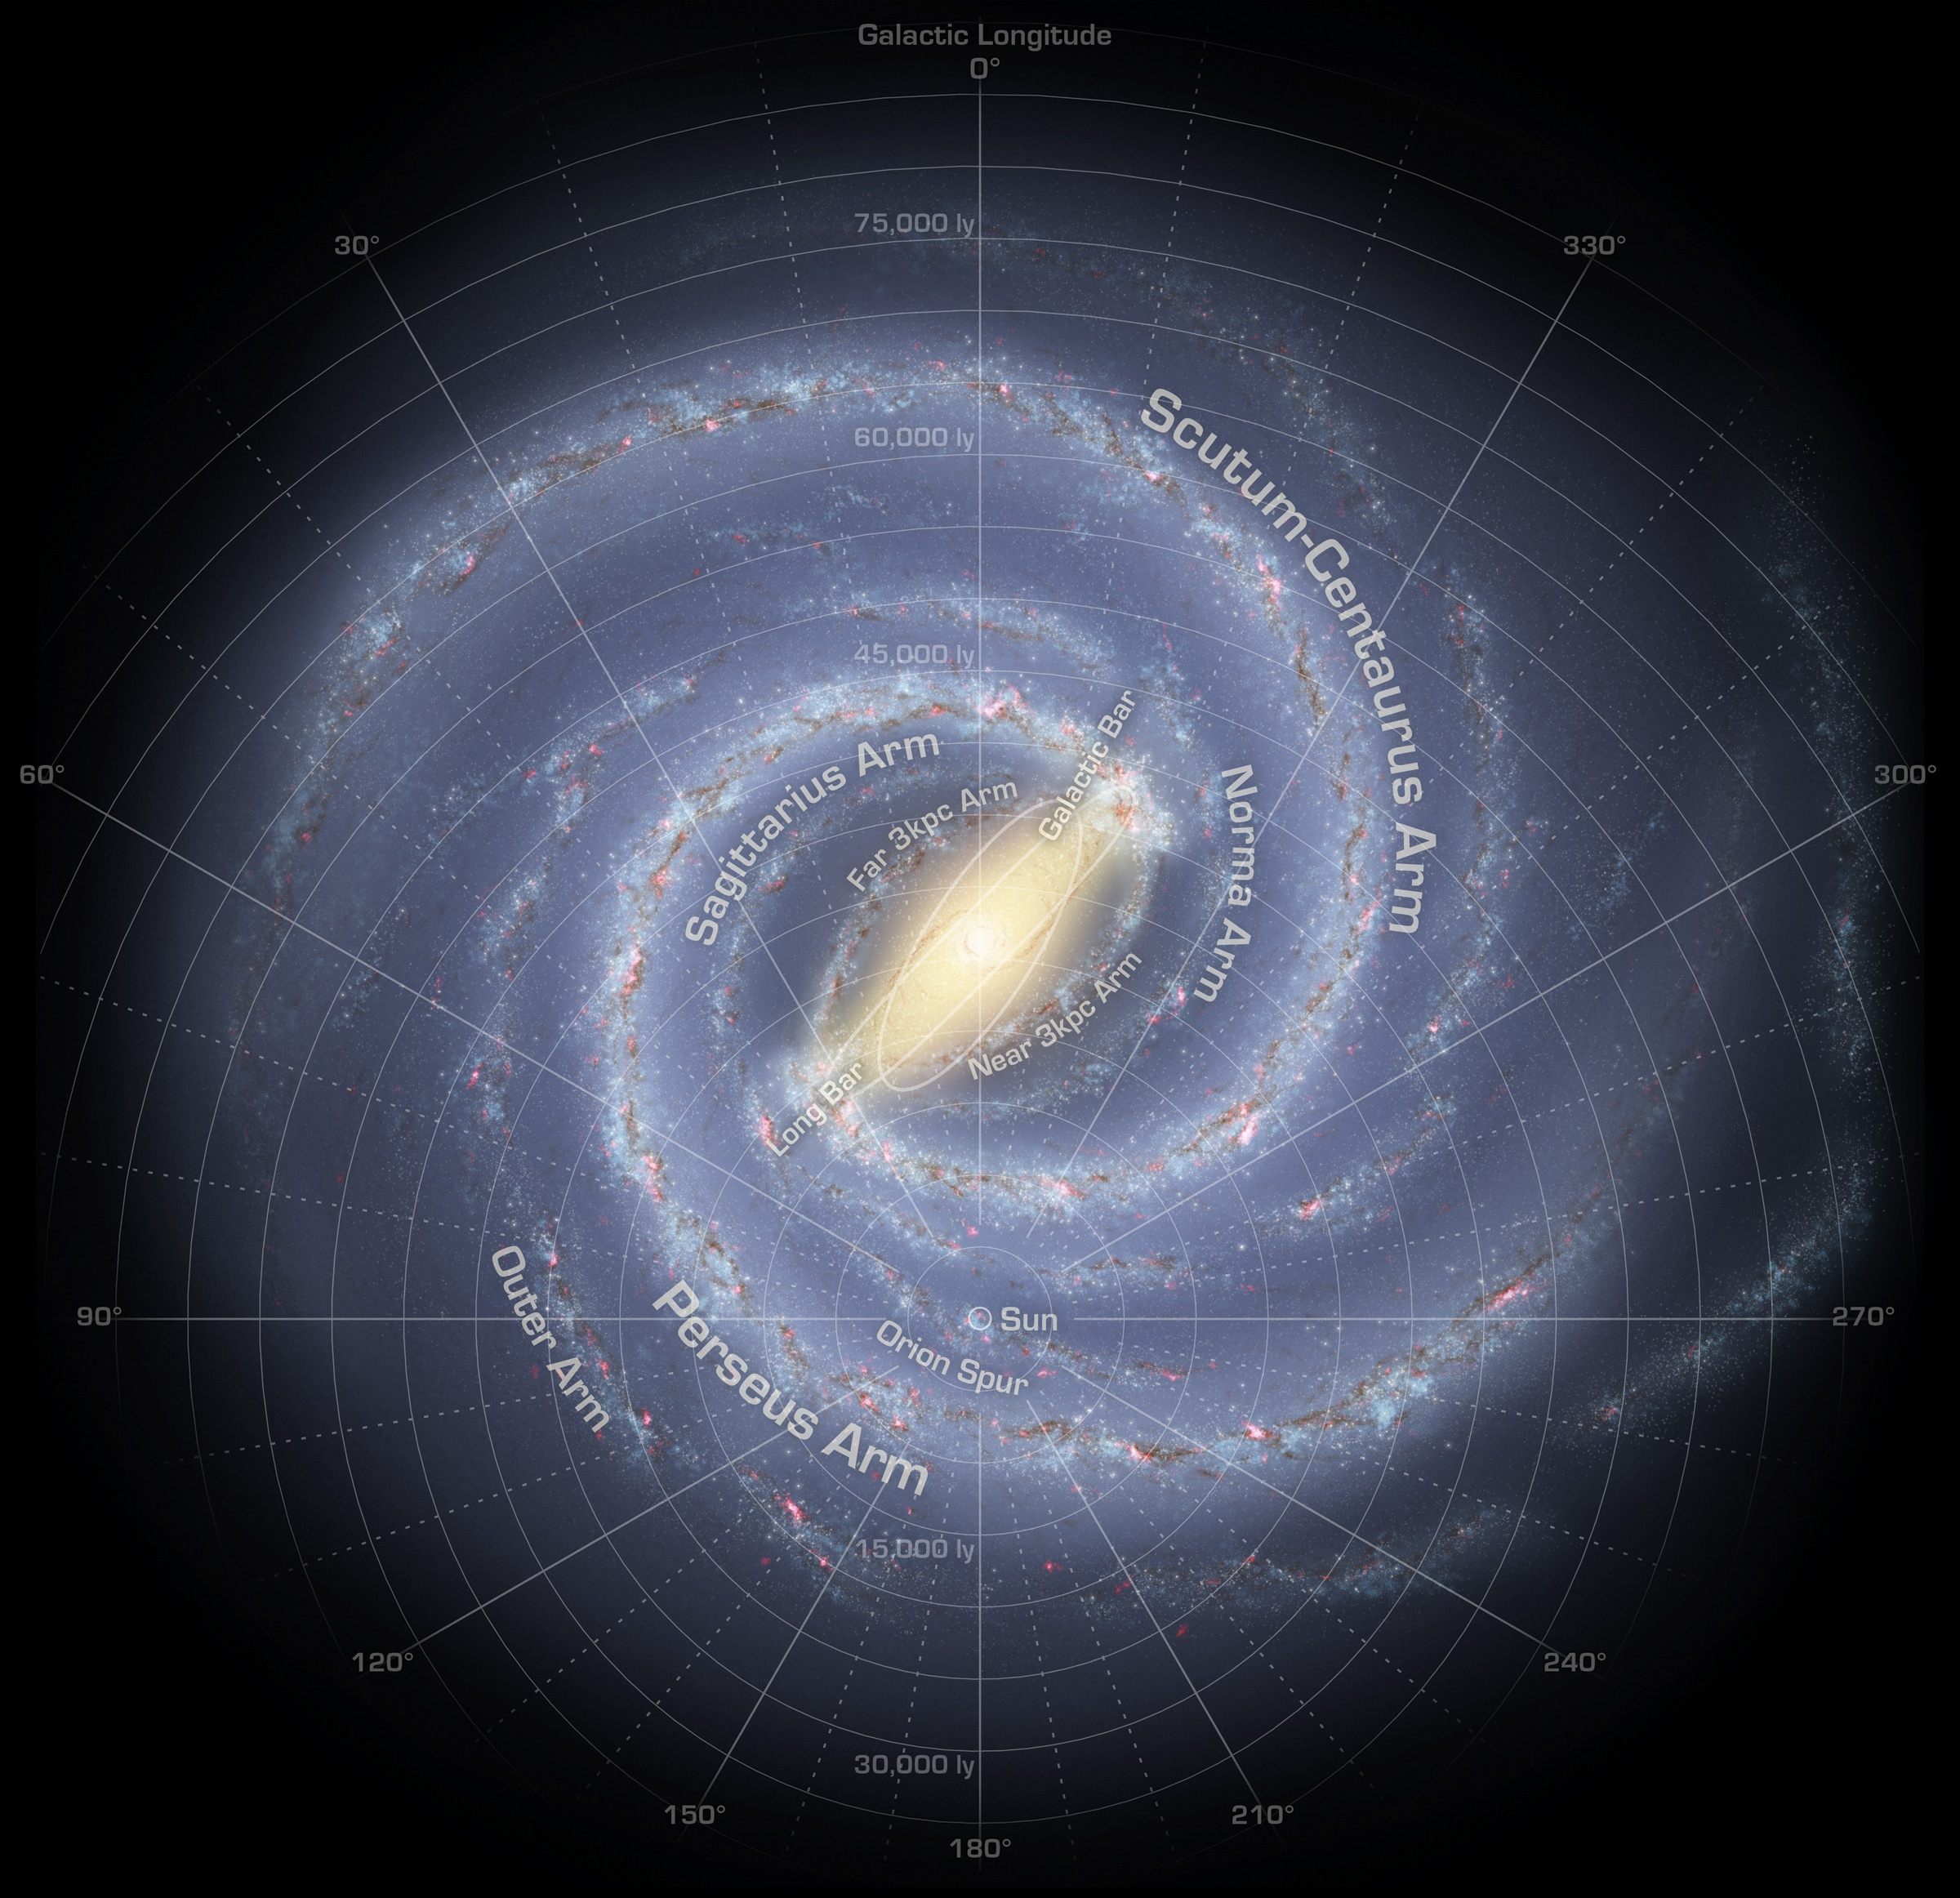
\includegraphics[width=\linewidth]{images/milkyway_structure_big_crop.jpeg}%
      \begin{tikzpicture}[overlay, remember picture, shift={(current page.center)}]%
        \only<1>{\draw[red!70!black, thick, o->] (-3.753, -1.41) -- +(65:4.5);}%
        \only<2>{\draw[red!70!black, thick, o->] (-3.819, -1.32) -- +(0:4.5);}%
      \end{tikzpicture}%
    \end{column}%
    \begin{column}{0.47\textwidth}%
      \begin{tikzpicture}%
        \begin{axis}[%
            title={$\TB$ für $l=\only<1>{\SI{335}{\degree}}\only<2>{\SI{270}{\degree}}$},
            xmin=21.09,
            xmax=21.12,
            ymin=-10,
            ymax=120,
            width=0.93\linewidth,
            xlabel={\SIQ{λ}{\centi\meter}},
            ylabel={$\SIQ{\TB}{\kelvin}$},
          ]%
          \only<1>{%
            \addplot[red!70!black] table[x index=3, y index=1]{./data/radial_velocity_l335.txt};%
          }
          \only<2>{%
          \addplot[red!70!black] table[x index=3, y index=1]{./data/radial_velocity_l270.txt};%
          }
        \end{axis}%
      \end{tikzpicture}%
    \end{column}%
  \end{columns}%
\end{frame}
